\documentclass[letterpaper, 12pt]{article}
\usepackage{pgfplots}

\pgfplotsset{compat=1.10}
\usepgfplotslibrary{fillbetween}
\usetikzlibrary{patterns}
\usetikzlibrary{calc}

\renewcommand*{\arcsin}{\sin^{-1}}
\renewcommand*{\arccos}{\cos^{-1}}
\renewcommand*{\arctan}{\tan^{-1}}
\newcommand*{\arccot}{\cot^{-1}}
\newcommand*{\arcsec}{\sec^{-1}}
\newcommand*{\arccsc}{\csc^{-1}}
\newcommand*{\diff}{\mathrm{d}}
\newcommand*{\Diff}[1]{\mathrm{d^#1}}
\newcommand*{\e}{\mathrm{e}}

\title{Volumes By Integration (Disks)}
\author{Alvin Lin}
\date{Calculus II: August 2016 - December 2016}

\begin{document}

\maketitle

\section*{Volumes By Integration (Disks)}

\begin{center}
  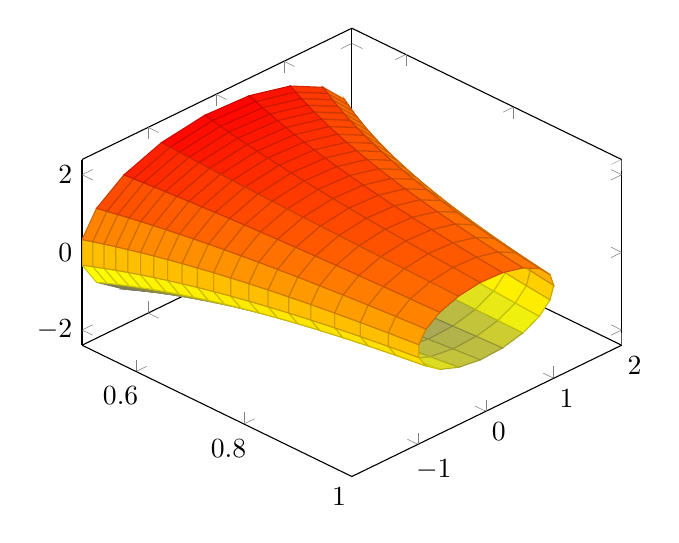
\begin{tikzpicture}
    \begin{axis}[view={45}{45}]
      \addplot3[
        surf,
        samples=20,
        domain=1:2,
        y domain=0:2*pi,
        z buffer=sort,
        ztick=\empty]
        (
          {1/x},
          {x * cos(deg(y))},
          {x * sin(deg(y))}
        );
   \end{axis}
  \end{tikzpicture}
\end{center}
We can take the volume of the above solid by taking areas of cross-sectional
slices (\( A_{i} \)) of the volume.
\[ V_{i} = A_{i}\Delta x \]
\[ V \approx \sum_{i=1}^{n}{A_{i}\Delta x} \approx \lim_{i=1}^{n}{V_{i}} \]
\[ V = \lim_{n \to \infty}\sum_{i=1}^{n}{V_{i}} = \int_{a}^{b}{A\diff{x}} \]

\subsection*{Example 1}
Find the volume of \( y = 1-x^{2} \) rotated about the x-axis.
\begin{center}
  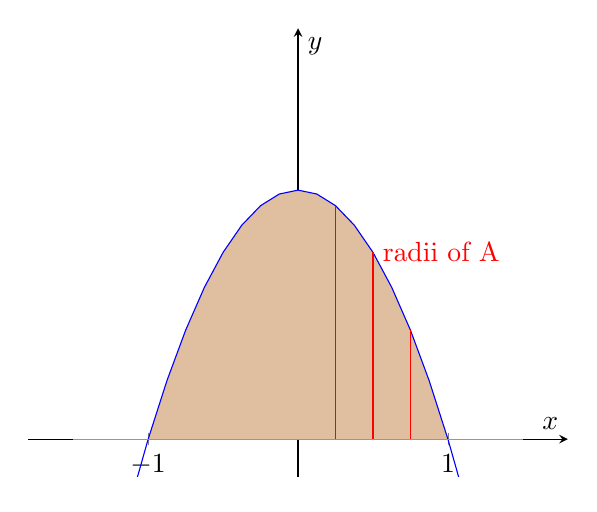
\begin{tikzpicture}
    \begin{axis}[axis lines=middle,
                 xlabel=\(x\), ylabel=\(y\),
                 ymin=0, ymax=1.5,
                 enlargelimits,
                 ytick=\empty,
                 xtick={-1,1}]
      \addplot[name path=F,
               blue,
               domain={-1.5:1.5}]{1-x^2} node[pos=1, below]
               {\(g\)};
      \addplot[name path=G, green, domain={-1.5:1.5}]{0};
      \addplot[name path=R1, red] coordinates {(0.25, 0) (0.25, 0.9375)};
      \addplot[name path=R1, red] coordinates {(0.5, 0) (0.5, 0.75)}
               node[pos=1, right]{radii of A};
      \addplot[name path=R1, red] coordinates {(0.75, 0) (0.75, 0.4375)};
      \addplot[color=brown!50] fill between [
               of=F and G, soft clip={domain=-1:1}];
    \end{axis}
  \end{tikzpicture}
\end{center}
\[ V = \int{A\diff{x}} \]
\[ V = \int{\pi r^{2}\diff{x}} \]
\[ V = \int_{-1}^{1}{\pi(1-x^{2})^{2}\diff{x}} \]
\[ V = \pi\int_{-1}^{1}{1-x^{4}-2x^{2}\diff{x}} \]
\[ V = \pi\bigg[x+\frac{x^{5}}{5}-\frac{2x^{3}}{3}\bigg]_{-1}^{1} \]
\[ V = \frac{16\pi}{15} \]

\subsection*{Example 2}
Find the volume of \( y = \ln(x) \) bounded by the lines \( y = 1 \),
\( y = 2 \), \( x = 0 \) when rotated about the y-axis.
\begin{center}
  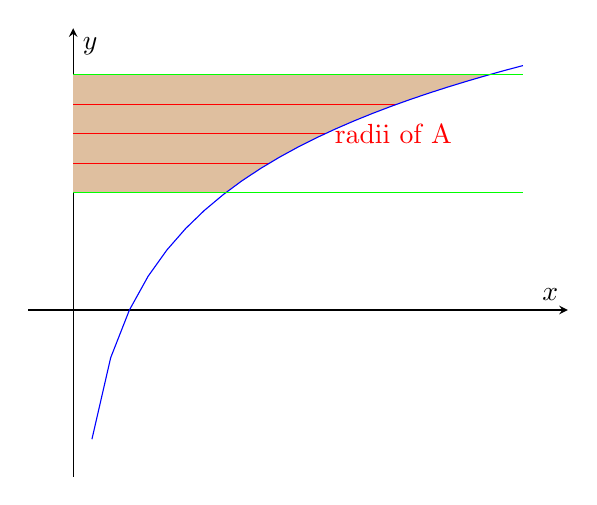
\begin{tikzpicture}
    \begin{axis}[axis lines=middle,
                 xlabel=\(x\),
                 ylabel=\(y\),
                 enlargelimits,
                 ytick=\empty,
                 xtick=\empty]
    \addplot[name path=A,
             red,
             domain={0:pow(e, 1.5)}]{1.5} node[pos=1, right]
             {radii of A};
    \addplot[name path=B, red, domain={0:pow(e, 1.25)}]{1.25};
    \addplot[name path=C, red, domain={0:pow(e, 1.75)}]{1.75};
    \addplot[name path=F, blue, domain={0:8}]{ln(x)};
    \addplot[name path=G, green, domain={0:8}]{1};
    \addplot[name path=H, green, domain={0:8}]{2};
    \addplot[color=brown!50] fill between [
             of=G and H, soft clip={domain=0:e}];
    \addplot[color=brown!50] fill between [
             of=F and H, soft clip={domain=e:e^2}];
    \end{axis}
  \end{tikzpicture}
\end{center}
\[ V = \int{A\diff{y}} \]
\[ V = \int{\pi r^{2}\diff{y}} \]
\[ V = \int_{1}^{2}{\pi(x)^{2}\diff{y}} \]
\[ V = \int_{1}^{2}{\pi(\e^{y})^{2}\diff{y}} \]
\[ V = \pi\int_{1}^{2}{\e^{2y}\diff{y}} \]
\[ V = \pi\bigg[\frac{\e^{2y}}{2}\bigg]_{1}^{2} \]
\[ V = \frac{\pi}{2}\bigg[\e^{4}-\e^{2}\bigg] \]

\subsection*{Example 3}
Find the volume of the region enclosed between \( y^{2} = x \) and
\( x = 2y \) when it is rotated about the y-axis.
\begin{center}
  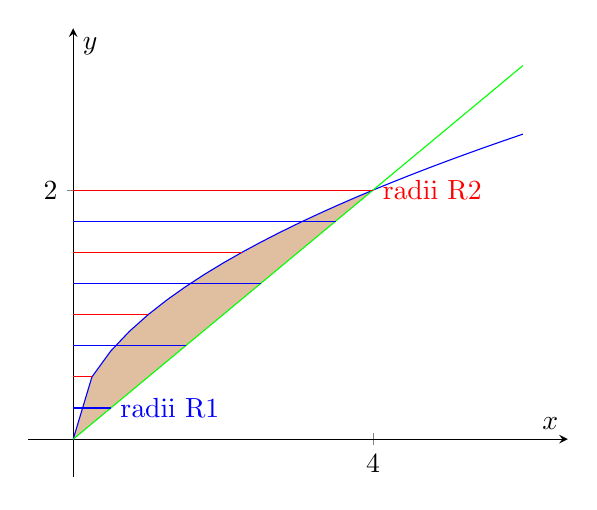
\begin{tikzpicture}
    \begin{axis}[axis lines=middle,
                 xlabel=\(x\),
                 ylabel=\(y\),
                 enlargelimits,
                 ytick={2},
                 xtick={4}]
    \addplot[name path=F, blue, domain={0:6}]{sqrt(x)};
    \addplot[name path=G, green, domain={0:6}]{x/2};
    \addplot[name path=B1, blue, domain={0:0.5}]{0.25} node[pos=1, right]
        {radii R1};
    \addplot[name path=B2, blue, domain={0:1.5}]{0.75};
    \addplot[name path=B3, blue, domain={0:2.5}]{1.25};
    \addplot[name path=B4, blue, domain={0:3.5}]{1.75};
    \addplot[name path=R1, red, domain={0:4}]{2} node[pos=1, right]
        {radii R2};
    \addplot[name path=R2, red, domain={0:2.25}]{1.5};
    \addplot[name path=R3, red, domain={0:1}]{1};
    \addplot[name path=R4, red, domain={0:0.25}]{0.5};
    \addplot[color=brown!50] fill between [
             of=F and G, soft clip={domain=0:4}];
    \end{axis}
  \end{tikzpicture}
\end{center}
\[ V = \int{A\diff{y}} \]
\[ V = \int{\pi(R1)^{2}-(R2)^{2}\diff{y}} \]
\[ V = \pi\int_{0}^{2}{(2y)^{2}-(y^{2})^{2}\diff{y}} \]
\[ V = \pi\int_{0}^{2}{4y^{2}-y^{4}\diff{y}} \]
\[ V = \pi\bigg[\frac{4y^{3}}{3}-\frac{y^{5}}{5}\bigg]_{0}^{2} \]
\[ V = \frac{32\pi}{3}-\frac{32\pi}{5} \]

\subsection*{Example 4}
\[ y = x^{2} \quad x = y^{2} \]
\begin{center}
  rotated about:
\end{center}
\[ x = -1 \]
\begin{center}
  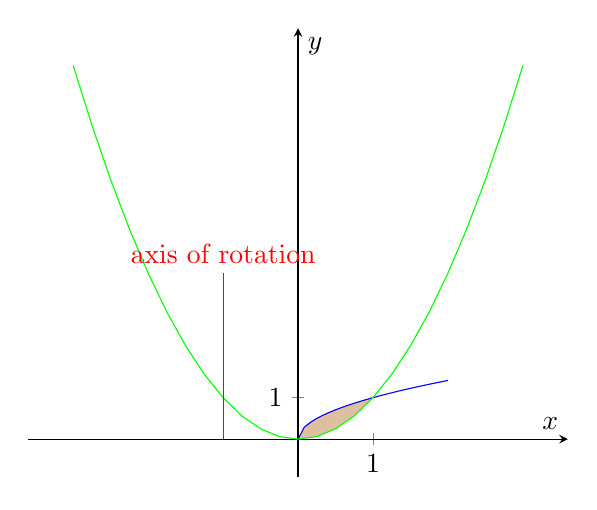
\begin{tikzpicture}
    \begin{axis}[axis lines=middle,
                 xlabel=\(x\),
                 ylabel=\(y\),
                 enlargelimits,
                 ytick={1},
                 xtick={1}]
    \addplot[name path=F, blue, domain={0:2}]{sqrt(x)};
    \addplot[name path=G, green, domain={-3:3}]{pow(x,2)};
    \addplot[name path=R1, red] coordinates {(-1, 0) (-1, 4)}
             node[pos=1, above] {axis of rotation};
    \addplot[color=brown!50] fill between [
             of=F and G, soft clip={domain=0:1}];
    \end{axis}
  \end{tikzpicture}
\end{center}
\[ V = \int{A\diff{y}} \]
\[ V = \int{\pi(R1)^{2}-(R2)^{2}\diff{y}} \]
\[ V = \pi\int_{0}^{1}{[(1+x)^{2}-(1+x)^{2}]\diff{y}} \]
\[ V = \pi\int_{0}^{1}{[(1+\sqrt{y})^{2}-(1+y^{2})^{2}]\diff{y}} \]
\[ V = \pi\int_{0}^{1}{[1+y+2\sqrt{y}-1-y^{4}-2y^{2}]\diff{y}} \]
\[ V = \pi\bigg[y+\frac{y^{2}}{2}+\frac{4y^{3/2}}{3}-
   y-\frac{y^{5}}{5}-\frac{2y^{3}}{3}\bigg] \]
\[ V = \frac{29\pi}{30} \]

\subsection*{Practice Problem 12}
\[ y = \e^{-x} \quad y = 1 \quad x = 2 \]
\begin{center}
  rotated about:
\end{center}
\[ y = 2 \]
\begin{center}
  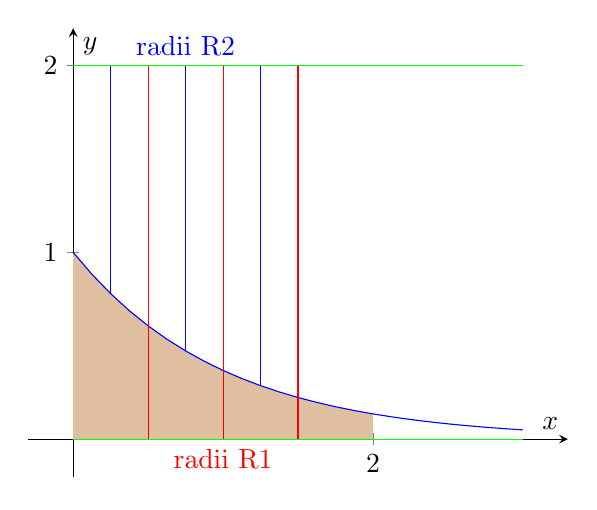
\begin{tikzpicture}
    \begin{axis}[axis lines=middle,
                 xlabel=\(x\),
                 ylabel=\(y\),
                 enlargelimits,
                 ytick={1,2},
                 xtick={2}]
    \addplot[name path=F, blue, domain={0:3}]{pow(e,-x)};
    \addplot[name path=G, green, domain={0:3}]{2};
    \addplot[name path=H, green, domain={0:3}]{0};
    \addplot[color=brown!50] fill between [
             of=F and H, soft clip={domain=0:2}];
    \addplot[name path=R1, red] coordinates {(0.5, 0) (0.5, 2)};
    \addplot[name path=R2, red] coordinates {(1, 0) (1, 2)}
             node[pos=0, below] {radii R1};
    \addplot[name path=R3, red] coordinates {(1.5, 0) (1.5, 2)};
    \addplot[name path=B1, blue] coordinates {(0.25, 0.7788) (0.25, 2)};
    \addplot[name path=B2, blue] coordinates {(0.75, 0.4723) (0.75, 2)}
             node[pos=1, above] {radii R2};
    \addplot[name path=B3, blue] coordinates {(1.25, 0.2865) (1.25, 2)};
    \end{axis}
  \end{tikzpicture}
\end{center}
\[ V = \int{A\diff{x}} \]
\[ V = \int{\pi(R1)^{2}-(R2)^{2}\diff{y}} \]
\[ V = \pi\int_{0}^{2}{[(2-y)^{2}-1^{2}]\diff{x}} \]
\[ V = \pi\int_{0}^{2}{[(2-\e^{-x})^{2}-1]\diff{x}} \]
\[ V = \pi\int_{0}^{2}{[4-\e^{-2x}-4\e^{-x}-1]\diff{x}} \]
\[ V = \pi\int_{0}^{2}{[3+\e^{2x}-4\e^{-x}]\diff{x}} \]
\[ V = \pi\bigg[3x+\frac{\e^{-2x}}{-2}+4\e^{-x}\bigg]_{0}^{2} \]
\[ V = \pi\bigg[(6-\frac{1}{2}\e^{-4}+4\e^{-2})-(\frac{-1}{2}+4)\bigg] \]

\subsection*{Volume of a Frustum}
\begin{center}
  \begin{tikzpicture}
    \begin{scope}
      \clip (-4,0) rectangle (4,2);
      \draw[dashed] (0,0) circle (4 and 1);
    \end{scope}
    \begin{scope}
      \clip (-4,0) rectangle (4,-2);
      \draw (0,0) circle (4 and 1);
    \end{scope}
    \draw (0,4) circle (2 and 0.5);
    \draw (-4,0) -- (-2,4);
    \draw (4,0) -- (2, 4);
    \draw[dashed] (4,0) -- node[above] {\( r \)}
                           coordinate[](a)(0,0)
                        -- node[left] {\( h \)}
                           coordinate[](b)(0,4)
                        -- node[left] {\( R \)}
                           coordinate[](c)(2,4);
  \end{tikzpicture}
\end{center}
We can turn this problem into an integration problem by taking a slice of the
frustum and revolving it around the x-axis.
\begin{center}
  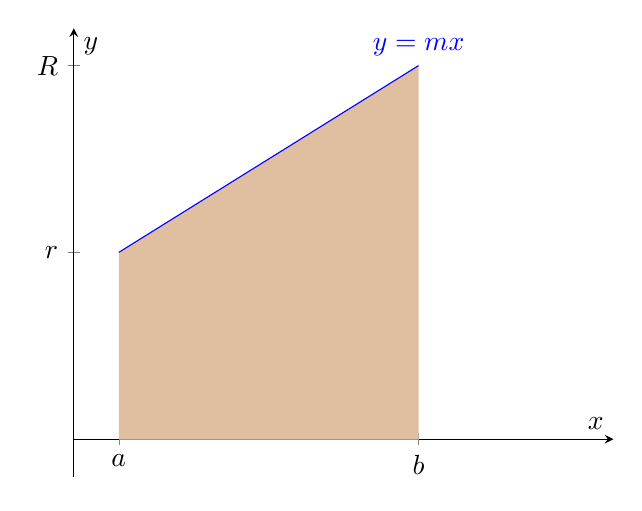
\begin{tikzpicture}
    \begin{axis}[axis lines=middle,
                 xlabel=\(x\),
                 ylabel=\(y\),
                 enlargelimits,
                 xtick={2,4},
                 xticklabels={\( a \), \( b \)},
                 ytick={2,4},
                 yticklabels={\( r \), \( R \)},
                 xmax=5]
    \addplot[name path=F,
             blue,
             domain={2:4}]{x} node[pos=1, above]
             {\( y=mx \)};
    \addplot[name path=G,
             green,
             domain={2:4}]{0} node[pos=1, left]
             {};
    \addplot[color=brown!50] fill between [
             of=F and G, soft clip={domain=2:4}];
    \end{axis}
  \end{tikzpicture}
\end{center}
\[ a-b = h \quad y = mx \]
\[ r = ma \quad R = mb \]
\[ V = \int{A\diff{x}} \]
\[ V = \int{\pi r^{2}\diff{x}} \]
\[ V = \pi\int_{a}^{b}{(y)^{2}\diff{x}} \]
\[ V = \pi\int_{a}^{b}{(mx)^{2}\diff{x}} \]
\[ V = \pi(m^{2})\bigg[\frac{x^{3}}{3}\bigg]_{a}^{b} \]
\[ V = \pi(m^{2})(\frac{b^{3}}{3}-\frac{a^{3}}{3}) \]
\[ V = \frac{\pi(m^{2})}{3}(b^{3}-a^{3}) \]
\[ V = \frac{\pi(m^{2})}{3}(b-a)(b^{2}+ab+a^{2}) \]
Since we know \( b-a = h \), \( r = ma \), and \( R = mb \):
\[ V = \frac{\pi(m^{2})h}{3}
   ((\frac{r}{m})^{2}+\frac{Rr}{m^{2}}+(\frac{R}{m})^{2}) \]
\[ V = \frac{\pi h}{3}[r^{2}+R^{2}+Rr] \]

\subsection*{Volume of a Section of a Sphere}
\begin{center}
  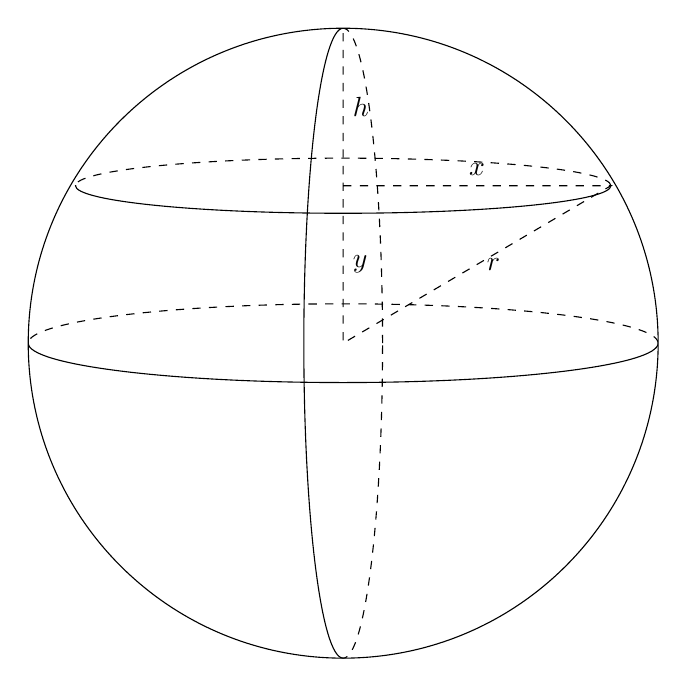
\begin{tikzpicture}
    \draw (0,0) circle (4);
    \begin{scope}
      \clip (0,-4) rectangle (1,4);
      \draw[dashed] (0,0) circle (0.5 and 4);
    \end{scope}
    \begin{scope}
      \clip (0,-4) rectangle (-1,4);
      \draw (0,0) circle (0.5 and 4);
    \end{scope}
    \begin{scope}
      \clip (-4,0) rectangle (4,1);
      \draw[dashed] (0,0) circle (4 and 0.5);
    \end{scope}
    \begin{scope}
      \clip (-4,0) rectangle (4,-1);
      \draw (0,0) circle (4 and 0.5);
    \end{scope}
    \begin{scope}
      \clip (-4,2) rectangle (4,3);
      \draw[dashed] (0,2) circle (3.4 and 0.35);
    \end{scope}
    \begin{scope}
      \clip (-4,2) rectangle (4,1);
      \draw (0,2) circle (3.4 and 0.35);
    \end{scope}
    \draw[dashed] (0,2) -- node[above] {\( x \)}
                           coordinate[](a)(3.4,2)
                        -- node[right] {\( r \)}
                           coordinate[](b)(0,0)
                        -- node[right] {\( y \)}
                           coordinate[](c)(0,2)
                        -- node[right] {\( h \)}
                           coordinate[](d)(0, 4);
  \end{tikzpicture}
\end{center}
The same proof as above can be applied to most shapes. For example, a section
of a sphere:
\begin{center}
  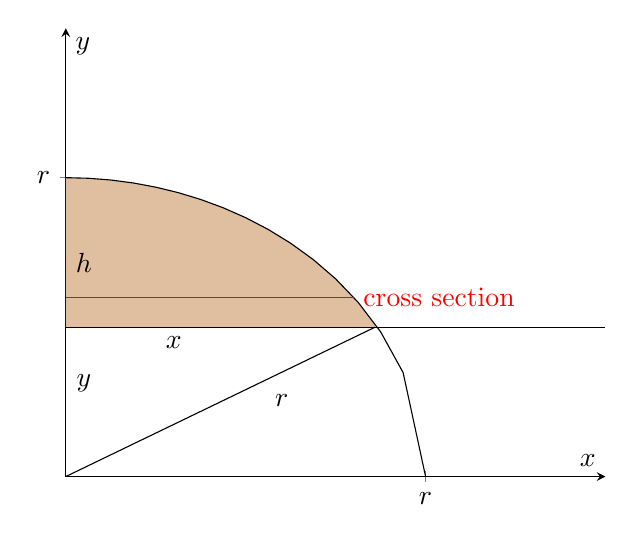
\begin{tikzpicture}
    \begin{axis}[axis lines=middle,
                 xlabel=\(x\),
                 ylabel=\(y\),
                 xtick={2},
                 xticklabels={\( r \)},
                 ytick={2},
                 yticklabels={\( r \)},
                 xmax=3,
                 ymax=3]
    \addplot[name path=F, black, domain={0:3}]{sqrt(4-x^2)};
    \addplot[name path=G, black, domain={0:3}]{1} node[pos=0.2, below]
        {\( x \)};
    \addplot[color=brown!50] fill between [
             of=F and G, soft clip={domain=0:1.72}];
    \addplot[black] coordinates {(0,0) (1.72,1)};
    \node[anchor=south] at (axis cs:1.2,0.4) {\( r \)};
    \node[anchor=south] at (axis cs:0.1,1.3) {\( h \)};
    \node[anchor=south] at (axis cs:0.1,0.5) {\( y \)};
    \addplot[name path=R4, red, domain={0:1.6}] {1.2}
             node[pos=1, right] {cross section};
    \end{axis}
  \end{tikzpicture}
\end{center}
From the Pythagorean theorem, we know that \( x^{2}+y^{2} = r^{2} \), thus it
follows that \( x^{2} = r^{2}-y^{2} \).
\[ V = \int{A\diff{y}} \]
\[ V = \int{\pi x^{2}\diff{y}} \]
\[ V = \int_{r-h}^{r}{\pi(r^{2}-y^{2})\diff{y}} \]
\[ V = \pi\bigg[r^{2}y-\frac{y^{3}}{3}\bigg]_{r-h}^{r} \]
\[ V = \pi(h^{2}r-\frac{h^{3}}{3}) \]
\[ V = \pi h^{2}(r-\frac{1}{3}h) \]

\begin{center}
  If any errors are found, please contact me at alvin.lin.dev@gmail.com
\end{center}

\end{document}
